\documentclass[12pt, a4paper]{article}

%==================================================
%wichtige Packages
%==================================================

\usepackage[T1]{fontenc}                %Richtige Darstellung Sonderzeichen
\usepackage[utf8]{inputenc}             %Richtige Darstellung Umlaute
\usepackage[ngerman]{babel}             %Sprache: Deutsch
\usepackage{helvet}                     %Schriftart: Helvetica
\usepackage[onehalfspacing]{setspace}   %Zeilenabstand: 1,5
\usepackage{import}                     %Import Datein
\usepackage{subfiles}                   %Unterkapitel
\usepackage{paralist}
\usepackage[hyphens]{url}               %Zeilenumbruch in URL
\usepackage[driver=pdftex]{geometry}    %Seitenränder
\usepackage[hang]{footmisc}             %Fußnote Strich unten
\usepackage{graphicx}                   %Für Bilder
\usepackage{longtable}                  %Abkürzungsverzeichnis
\usepackage{tocloft}                    %Anhangsverzeichnis
\usepackage{titlesec}                   %Anhangsverzeichnis
\usepackage{titletoc}                   %Anhangsverzeichnis
\usepackage{etoolbox}                   %Anhangsverzeichnis
\usepackage{csquotes}
\usepackage[
  style=authoryear, 
  urldate=long, 
  maxbibnames=99
  ]{biblatex}                             %Literaturverzeichnis
\usepackage[
   disable
  ]{todonotes}                            %Todos
\usepackage[hidelinks]{hyperref}        %hidelinks versteckt den roten Kasten
\usepackage{nameref}% loads gettitlestring
\usepackage{array}
\usepackage[labelfont={color=gray,small},textfont={color=gray,small}]{caption}

%==================================================
%Literaturverzeichnis
%==================================================

\addbibresource{Quellen.bib}

\DeclareDelimFormat{multinamedelim}{\addcomma\space}
\DeclareDelimFormat{finalnamedelim}{\addcomma\space}
\DeclareFieldFormat{title}{#1}
\DeclareFieldFormat{url}{#1}
\DefineBibliographyStrings{german}{%
  andothers = {et\addabbrvspace al\adddot},
}
\DeclareFieldFormat{extradate}{{\mknumalph{#1}}}
\DeclareNameAlias{sortname}{family-given}

\AtBeginBibliography{%
  \renewcommand*{\multinamedelim}{\addspace\slash\addspace}%
  \renewcommand*{\finalnamedelim}{\addspace\slash\addspace}%
}

% Fußnotenformat
\renewbibmacro{cite}{\printtext[bibhyperref]{\printnames{labelname} (\iffieldundef{year}{o. J.}{\printfield{year}}\printfield{extradate})}}

% Formatierung des Literaturverzeichnisses
% Website
\DeclareBibliographyDriver{online}{%
  \textbf{\printnames{author} (\iffieldundef{year}{o. J.}{\printfield{year}}\printfield{extradate}):}\newline%
  \textnormal{\printfield{title}}, \printfield{url}, \printfield{note}.\bigbreak}

% Paper
\DeclareBibliographyDriver{booklet}{%
  \textbf{\printnames{author} (\iffieldundef{year}{o. J.}{\printfield{year}}\printfield{extradate}):}\newline%
  \textnormal{\printfield{title}}.\bigbreak}

% Buch
\DeclareBibliographyDriver{book}{%
  \textbf{\printnames{author} (\iffieldundef{year}{o. J.}{\printfield{year}}\printfield{extradate}):}\newline%
  \textnormal{\printfield{title}}, \iffieldundef{edition}{o. A.}{\printfield{edition}}, \printlist{publisher}\iflistundef{location}{}{, \printlist{location}}.\bigbreak}     
%==================================================

% \paragraph and \subparagraph for forth and fifth level headings

\setcounter{secnumdepth}{5}
\setcounter{tocdepth}{4}

\titleformat{\paragraph}
    {\normalfont\normalsize\bfseries}{\theparagraph}{1em}{}
\titlespacing*{\paragraph}
    {0pt}{3.25ex plus 1ex minus .2ex}{1.5ex plus .2ex}

\titleformat{\subparagraph}
    {\normalfont\normalsize\bfseries}{\thesubparagraph}{1em}{}
\titlespacing*{\subparagraph}
    {0pt}{3.25ex plus 1ex minus .2ex}{1.5ex plus .2ex}



    \newcommand{\footappendix}[2]{
      \footnote{
        #1 \hyperref[#2]{\nameref*{#2}, S. \pageref*{#2}}.
      }
    }


%==================================================
%Einstellung Seitenränder
%==================================================
\geometry{
        left=4cm,
        right=2cm,
        top=2cm,
        bottom=2cm
    }
%==================================================

%==================================================
% Todos
%==================================================
\newcommand\todoin[2][]{\todo[inline, caption={2do}, #1]{
 \begin{minipage}{\textwidth-4pt}#2\end{minipage}}}

% Todos to left side
\reversemarginpar

% Todos Width
\setlength{\marginparwidth}{3.5cm}

% Todos Color
\definecolor{NOTES}{HTML}{00ffff}
\definecolor{REVIEW}{HTML}{d400ff}
\definecolor{TODO}{HTML}{90EE90}
%==================================================

%Variable zum speichern der Seite
\newcounter{savepage}

\begin{document}

    \newcounter{romanSection} % Inhaltsverzeichnis, etc, Mit Anhang
    \newcounter{romanPage}    % Inhaltsverzeichnis, etc, ohne Anhang


    %==================================================
    %Deckblatt + Sperrvermerk
    %==================================================

    {\pagestyle{empty}

    %=============================================================
%Deckblatt
%=============================================================

\noindent
\textbf{Name:} Tobias Binnewies

\bigbreak
\bigbreak
\bigbreak
\bigbreak
\bigbreak
\bigbreak
\bigbreak
\bigbreak


\noindent
\textbf{Hochschule Weserbergland} \\
Studiengang: Wirtschaftsinformatik (B. Sc.) \\
Studiengruppe: WI67/21 \\
Dozent: Ralf Hesse

\bigbreak
\bigbreak
\bigbreak
\bigbreak
\bigbreak
\bigbreak
\bigbreak
\bigbreak

\noindent
\textbf{Lösungsorientierte Transferarbeit 2 - Semester 5} \\
Bearbeitungszeitraum: 04.12.2023 bis 31.01.2024

\bigbreak
\bigbreak
\bigbreak
\bigbreak

\noindent
\textbf{Thema:} \\
Eignungsanalyse von Distributed Ledger Systemen in der Finanz Informatik GmbH \& Co. KG

\bigbreak
\bigbreak
\bigbreak
\bigbreak

\noindent
\textbf{Praxispartner:} \\
Finanz Informatik GmbH \& Co. KG \\
Laatzener Straße 5, 30539 Hannover

\bigbreak

\newpage

%\addtocontents{toc}{\cftpagenumbersoff{section}}
\cftaddtitleline*{toc}{section}{Deckblatt}{}

    }
    \newpage

    % {\pagestyle{empty}

    % \input{Sperrvermerk.tex}

    % }
    % \newpage


    %==================================================
    %Inhaltlsverzeichnis
    %==================================================
    
    {   
        %Kapitel und Seitennummerierung wird auf Römisch 1 gesetzt
        \setcounter{page}{1}
        \renewcommand{\thesection}{\Roman{section}}
            \pagenumbering{Roman}

    %Übershrift: Inhaltsverzeichnis
    \section{Inhaltsverzeichnis}        

    %Befehl, damit Inhaltsverzeichnis nicht doppelt da steht 
    \renewcommand{\contentsname}{}

    %Befehle zur Strukturierung des Inhaltsverzeichnisses (Anordnung)
    \setlength\cftbeforesecskip{3pt}
    \renewcommand{\cftsecleader}{\cftdotfill{\cftdotsep}}

    %Inhaltsverzeichnis wird erzeugt
    \tableofcontents 

    \newpage


    %==================================================
    %Abkürzungsverzeichnis
    %==================================================
    
    \input{Abkürzungsverzeichnis.tex}    

    \newpage
    

    %==================================================
    %Abbildungsverzeichnis
    %==================================================

    %Überschrift: Abbildungsverzeichnis
    \section{Abbildungsverzeichnis}

    %Befehl, damit Abbildungsverzeichnis nicht doppelt da steht 
    \renewcommand{\listfigurename}{}

    %Abbildungsverzeichnis wird erzeugt
    \listoffigures                      

    }

    % KapitelNummerierung merken
    \setcounter{romanSection}{\thesection}
    \setcounter{romanPage}{\arabic{page}}

    \newpage

    
    %==================================================
    %Inhaltliches
    %==================================================

    {
        % KapitelNummerierung auf 0 setzen und mit arabischen Zahlen belegen
        \setcounter{section}{0}
        \setcounter{page}{1}
            \pagenumbering{arabic}

    %Hier steht der Inalt


    \renewcommand{\figurename}{Abb.}

    %Beispiel: \input{Grundlagen eines Netzwerks.tex}
    
\noindent %um die Einrückung zu löschen

\section{Einleitung}

% NOTES Einleitung:
% - Es wird auf den Zahlungsverkehr eingegangen
% - Es wird im Scope einer Bank betrachtet, nicht im Scope des gesamten Zahlungsverkehrs / Finanzsystems

Einleitung hier
\bigbreak

    
    \noindent
\section{Theorie}

% REVIEW Keine Wertung in diesem Kapitel, erst dann in Eignungsanalyse
% TODO Genauer erklären

\textcolor{red}{TODO Keine Wertung in diesem Kapitel, erst dann in Eignungsanalyse\break TODO Genauer Erklären}

\noindent

\subsection{Distributed Ledger System}
\label{sec:definition-dls}

\subsubsection{Distributed Ledger}
\label{sec:definition-distributed-ledger}
Ein Distributed Ledger ist eine Datenbank, die im Konsens geteilt und über ein Netzwerk synchronisiert wird, das sich über mehrere Standorte, Institutionen oder Länder erstreckt.\footcite[Vgl. hierzu und im Folgenden][]{w1,w2} 
Es ermöglicht, dass Transaktionen und Aufzeichnungen öffentlich und überprüfbar sind, und da es dezentralisiert ist, gibt es keinen einzelnen Ausfallpunkt. 
Jeder Teilnehmer im Netzwerk hat Zugang zu den Aufzeichnungen, die über dieses Netzwerk geteilt werden, und kann eine identische Kopie der Daten haben. Änderungen oder Ergänzungen am DL werden nahezu in Echtzeit in allen Kopien widergespiegelt, was die Transparenz und Sicherheit erhöht.
\bigbreak
\noindent
Ein Distributed Ledger System ist ein System, das einen Distributed Ledger verwendet, um Transaktionen zwischen Teilnehmern zu verwalten. Am häufigsten wird die Blockchain-Technologie als DL verwendet.\footcite[Vgl.][]{w3}

\subsubsection{Blockchain}
\label{sec:definition-blockchain}
\textcolor{red}{REVIEW evtl. ausführlicher}
Eine Blockchain ist eine spezielle Form eines Distributed Ledgers, die aus einer Kette von Blöcken besteht, die jeweils die zu speichernden Daten enthalten.\footcite[Vgl.][16]{q3} 
Ein Block besteht aus einem Header und einem Body.\footcites[Vgl. hierzu und im Folgenden][S. 161 ff\adddot]{q5}[]{w9}
\bigbreak
\noindent
Der Header enthält u. a. den Hash des vorherigen Blocks, einen Zeitstempel und die Nummer des Blocks.
Außerdem enthält der Header einen Hash des Bodys.
So wird gewährleistet, dass die Blöcke - und so auch die darin beinhalteten Daten - nach ihrem Eintrag nicht verändert werden können, ohne alle nachfolgenden Blöcke abzuändern. 
(So wird von „Block-Confirmation” gesprochen, wenn eine bestimmte Anzahl von Blöcken nach diesem Block hinzugefügt wurden - je mehr desto sicherer -, da er erst dann als „unveränderlich” gilt.\footcites[Vgl.][191]{q5})
\bigbreak
\noindent
Der Body enthält die eigentlichen Daten, die gespeichert werden sollen. Im Falle einer Kryptowährung sind dies bspw. die Transaktionen, die in diesem Block gespeichert werden.

\subsubsection{Kryptowährung}
\label{sec:definition-kryptowaehrung}
Ein DLS kann viele Anwendungsmöglichkeiten haben. Am wohl bekanntesten ist die Verwendung als Kryptowährung, wie bspw. Bitcoin.\footcite[Vgl. hierzu und im Folgenden][1]{q4} 
Hierbei werden die Transaktionen zwischen den Teilnehmern des Netzwerks durchgeführt, die in einer Blockchain festgehalten werden. 
So können Transaktionen Peer-to-Peer durchgeführt werden, also ohne dass eine zentrale Instanz diese überprüfen muss, da die Korrektheit der Transaktionen von allen Teilnehmern geprüft werden.
\bigbreak
\noindent
Bestimmste Chains - wie EVM-Chains - heben dieses Konzept auf eine neue Ebene, indem sie es ermöglichen, Smart Contracts zu erstellen.

\subsubsection{Ethereum Virtual Maschine Chain}
\label{sec:definition-evm-chain}
Eine EVM-Chain ist eine Blockchain-Netzwerk, das die Ethereum Virtual Machine (EVM) verwendet, um Smart Contracts auszuführen.\footcite[Vgl. hierzu und im Folgenden][]{w5}
Ethereum selbst ist eine EVM-Chain, die die Kryptowährung Ether (ETH) verwendet. Allerdings gibt es noch weitere Chains, die ebenfalls kompatibel mit der EVM sind, wie bspw. Binance Smart Chain (BSC) oder Polygon (MATIC)\footcite[Vgl.][]{w6}.
So kann für jede dieser Chains der gleiche Code - sowie Tools für dessen Entwicklung - verwendet werden, um Smart Contracts zu erstellen, die dann auf der jeweiligen Chain ausgeführt werden.

\subsubsection{Smart Contracts}
\label{sec:definition-smart-contracts}

Smart Contracts (im Sinne von Ethereum) sind Programme, die auf der Ethereum-Blockchain ausgeführt werden.\footcite[Vgl. hierzu und im Folgenden][]{w4} 
Sie bestehen aus einer Sammlung von Code (ihre Funktionen) und Daten (ihr Zustand), die - ebenso wie ein Benutzer-Wallet - an einer bestimmten Adresse auf der Ethereum-Blockchain (oder einer anderen EVM-Chain - S. \ref{sec:definition-evm-chain}) residieren.
Smart Contracts sind eine Art von Ethereum-Konto, was bedeutet, dass sie ein Guthaben haben und Ziel von Transaktionen sein können. 
Sie werden jedoch nicht von einem Benutzer kontrolliert, sondern sind im Netzwerk bereitgestellt und laufen wie programmiert. 
Benutzerkonten können dann mit einem Smart Contract interagieren, indem sie Transaktionen einreichen, die eine auf dem Smart Contract definierte Funktion ausführen. 
Außerdem können Regeln / Bedingungen definiert werden, nach den Code automatisch durchgeführt wird.
Standardmäßig können Smart Contracts nicht gelöscht werden, und Interaktionen mit ihnen sind irreversibel.

% TODO Nodes erklären
\subsubsection{Nodes}
\label{sec:definition-nodes}
Teilnehmer des Netzwerks, die über die gesamte Blockchain verfügen und die Transaktionen und Blöcke validieren werden Nodes genannt.\footcites[Vgl. hierzu und im Folgenden][]{w12}[]{w13} 
Diese Nodes formen das dezentralisierte Netzwerk, das die Blockchain betreibt.
Diese sind es auch, die den Code der Smart Contracts und die Transaktionen ausführen.
Außerdem validieren sie die Transaktionen und Blöcke, die von anderen Nodes erstellt wurden, und erstellen neue Blöcke, die sie dann an das Netzwerk senden.
Dazu verwenden sie einen Konsensalgorithmus, der bestimmt, welche Blöcke gültig sind (s. \ref{sec:definition-konsensalgorithmus}). 
Sowohl für das Ausführen der Smart Contracts als auch für das Validieren der Blöcke erhalten die Nodes eine Belohnung in Form von ETH (oder einer anderen Kryptowährung, je nach Chain), diese Belohnung wird Gas genannt.

% TODO Gas erklären
\subsubsection{Gas Fee}
\label{sec:definition-gas-fee}

\subsubsection{Konsensalgorithmus}
\label{sec:definition-konsensalgorithmus}
Um sicherzustellen, dass bestehende Blöcke nicht verändert werden können und der Inhalt neuer Blöcke valide ist, wird ein Konsensalgorithmus verwendet.\footcite[Vgl.][S. 2 f\adddot]{q4}
Die bekanntesten Algorithmen sind:
\begin{itemize}
    \item \textbf{Proof of Work (PoW):}
    Miner (Nodes) konkurrieren miteinerander, um ein mathematisches Problem zu lösen.\footcite[Vgl. hierzu und im Folgenden][3]{q4}
    Dem ersten, dem dies gelingt, erhält die Blockbelohnung und kann den nächsten Block erstellen.
    Um einen Block zu erstellen wird also Zeit benötigt, ein Angreifer müsste also eine höheren Rechenleistung als die Hälfte des Netzwerks besitzen, um die Blockchain zu manipulieren.

    \item \textbf{Proof of Stake (PoS):}
    Es wird zufällig eine Node ausgewählt, die den nächsten Block erstellen darf und so die Belohnung erhält.\footcite[Vgl. hierzu und im Folgenden][2]{q7}
    Es muss vorab eine Sicherheitsleistung (Stake) hinterlegt werden, die verloren geht, wenn die Node versucht, die Blockchain zu manipulieren. 
    Je höher der Stake, desto höher die Wahrscheinlichkeit, dass die Node ausgewählt wird.
    So wird verhindert, dass ein Angreifer die Blockchain manipuliert, da er mehr als die Hälfte des Stakes besitzen müsste, um die Blockchain zu manipulieren.

    \item \textbf{Proof of Authority (PoA):}
    Es wird eine Liste von Nodes festgelegt, die die Blockchain validieren dürfen.\footcite[Vgl. hierzu und im Folgenden][]{w14}
    Dieser Algorithmus wird häufig bei privaten Chains verwendet, da den Nodes vertraut werden muss.
    So kann die Blockchain nicht manipuliert werden, ohne dass eine der Nodes dies zulässt.
    Dieser Algorithmus ist sehr schnell, da keine Rechenleistung benötigt wird oder eine Auswahl getroffen werden muss, um einen Block zu erstellen.
    
\end{itemize}

% TODO Unterscheid zwischen Account- und Transactions-basierten Chains erklären
% --> Account-based Problem: Keine HD-Wallets einfach möglich, so weniger Anonymität
\subsubsection{Account-based vs. UTXO-based Chains}
\label{sec:definition-account-based-vs-utxo-based-chains}
\textcolor{red}{--> Account-based Problem: Keine HD-Wallets einfach möglich, so weniger Anonymität}

\subsubsection{ERC20 Token}
\label{sec:definition-erc20-token}
Es gibt diverse Standarts für Smart Contracts, die bestimmte Funktionen und Eigenschaften definieren.
Einer dieser Standarts ist der ERC20 Token Standard, der die Schnittstellen eines Smart Contracts definiert, der als Token verwendet werden soll.\footcite[Vgl. hierzu und im Folgenden][]{w7}
Ein Token kann dabei eine beliebige Repräsentation eines Vermögenswertes sein.
In diesem Smart Contract wird die Anzahl der Token gespeichert, die eine bestimme Adresse (also Benutzer-Wallet oder Smart Contract) besitzt.
Außerdem werden Funktionen definiert, um u. a. Token von einer Adresse zu einer anderen zu versenden, die Anzahl der Token einer Adresse abzufragen und anderen Adressen die Erlaubnis zu erteilen, Token von der eigenen Adresse zu versenden.\footcites[Vgl.][]{w8}[]{w7}

% TODO Layer 2 Solutions erklären
\subsubsection{Layer 2 Lösungen}
\label{sec:definition-layer-2-solutions}

% TODO EIP-712 / EIP-2612 / Relaying / Meta Transactions erklären
\subsubsection{Transaction Relayers}
\label{sec:definition-transaction-relayers}
\textcolor{red}{EIP-712 / EIP-2612 / Relaying / Meta Transactions erklären}

% REVIEW Sicherheitsrisiken wie Reentrancy / Oracle / etc. Attack? - i.V.m. Audit 
\subsubsection{Sicherheitsrisiken}
\label{sec:definition-sicherheitsrisiken}
\textcolor{red}{Sicherheitsrisiken wie Reentrancy / Oracle / etc. Attack? - i.V.m. Audit }


% REVIEW Proxys?
\subsubsection{Proxies}
\label{sec:definition-proxies}
\noindent

\subsection{Use Case Zahlungsverkehr}

\subsubsection{Zahlungsverkehr}

% NOTES Zahlungsverkehr:
% - Je nach Aufbau kann nur der Kontoinhaber selbst eine Transaktion vornehmen
% - Transaktionen können nicht rückgängig gemacht werden --> Rückbuchung durch erneute Transaktion
% - Transaktionen können nicht verändert werden --> Keine Manipulation möglich
% - AuditLog ist automatisch durch Technologie vorhanden
% - Durch Smart Contracts können bestimmte Finanzprodukte (z.B. Sparverträge, Kredite, ...) oder auch Multisign (per Multisign Contracts) abgebildet werden und so automatisiert werden

% Probleme:
% - Transaktionen sind öffentlich einsehbar --> Keine Privatsphäre (außer evtl. durch HD-Wallets)
% - Euro keine Kryptowährung --> Umwandlung in Token (Layer2) notwendig
% - Weiterentwicklung bei bspw. neuen Anforderungen schwierig --> Durch Proxys möglich

% REVIEW QUELLEN!
Ein Use Case dieser Technologie in Bereich einer Bank wäre der Zahlungsverkehr. So wird die Blockchain als Datenbank für die Konten der Kunden verwendet.
Eine Blockchain erfüllt automatisch durch ihren Aufbau einige Anforderungen an den Zahlungsverkehr, die in herkömlichen Systemen beachtet und umgesetzt werden müssen. So können Transaktionen - also in diesem Fall Einträge in diese Datenbank - nicht rückgängig, nicht verändert und so nicht manipuliert werden. Es gäbe dennoch die Möglichkeit - je nach konkreter Implementierung - bestimmte Sicherheitsmechanismen einzubauen, um bspw. gegen Geldwäsche oder fehlerhaft Buchungen vorzugehen. % TODO Ausführlicher & Besipiele / konkrete Idee der Implementierung
Außerdem ist ein AuditLog automatisch vorhanden, da alle Transaktionen in der Blockchain gespeichert werden.
Aufbauend darauf können Smart Contracts verwendet werden, um bestimmte Finanzprodukte (z.B. Sparverträge, Kredite, ...) oder auch Multisign (per Multisign Contracts) abzubilden und so zu automatisieren. % TODO Ausführlicher & Besipiele / konkrete Idee der Implementierung
%...
Um den Kontostand eines Kunden widerzuspiegeln, gäbe es mehrere Möglichkeiten:
% REVIEW andere Begriffe für Layer 1 und Layer 2 Währung (ERC20 Token, ...)
\begin{itemize}
    \item Wert als Layer 1 Währung (z.B. ETH) wechseln
    \item Wert als bestehende Layer 2 Währung (z.B. Stablecoin) wechseln
    \item Wert als eigene Layer 2 Währung wechseln
\end{itemize}
Das Problem bei einer Layer 1 Währung ist, dass diese nicht den Euro darstellt. So müsste der Wert immer in eine andere Währung umgerechnet werden, was zu zusätzlichen Kosten führt. Außerdem ist der Wert einer Layer 1 Währung sehr volatil, was zu Problemen führen kann, wenn der Wert des Kontos nicht mit dem Wert der Layer 1 Währung übereinstimmt.
Eine Layer 2 Währung, die den Euro darstellt, wäre ein Stablecoin. Dieser ist an den Euro gekoppelt und hat somit immer den gleichen Wert. 
Das Problem daran - sowie auch bei der Layer 1 Währung - ist, dass diese einen tatsächlichen Wert haben, und so die Bank dieses Geld nicht für eigene Geschäfte verwenden kann.
So währe eine eigene Layer 2 Währung sinnvoll, um den Wert eines Kontos darzustellen, ohne dass dieser einen tatsächlichen Wert hat. So kann die Bank diesen Wert für eigene Geschäfte verwenden, ohne dass der Kunde dadurch einen Verlust erleidet. Außerdem kann so gewährleistet werden, dass nur Kunden der Bank diesen Token verwenden können, da die Bank die einzige ist, die diesen Token ausgibt.
\bigbreak

\noindent

\subsection{Öffentliches vs. privates Netzwerk}
\label{sec:oeffentlich-vs-privates-netzwerk}



    \noindent
\section{Use Case - Zahlungsverkehr}

% \noindent

\subsection{Bewertungskriterien}

\todoin[color=NOTES]{
Kriterien: \break
- Perfomance (Schnelligkeit) --> Durch Layer 2 Lösungen (z.B. Lightning Network) (recht) hoch, ansonsten durch privates System (dann aber nicht dezentral und so Sicherheitsrisiken) \break
- Skalierbarkeit --> Durch Layer 2 Lösungen (z.B. Lightning Network) möglich \break
- Sicherheit (u.a. AuditLog) --> Wenn öffentliches System, dann generell durch Implementeirung beeinflusst, ansonsten durch privates System wie jetzt \break
- Transparenz --> In öffentlichem System sehr hoch, ansonsten durch privates Systeme wie jetzt \break
- Privatsphäre --> In öffnetlichem System quasi nicht möglich (evtl. durch HD-Wallets), ansonsten durch privates System (dann aber nicht dezentral und so Sicherheitsrisiken) \break
- Kosten  \break
- Komplexität (Aufwand, Wartung, ...) --> Erstmal Aufwand, dann aber gringer (vor allem wenn nur ein System verwendet wird, im Gegensatz zur aktuellen Situation) \break
- Erweiterbarkeit (z.B. neue Anforderungen) --> Durch Proxys möglich \break
}

\todoin[color=NOTES]{
    Ist-Zustand: \break
Quelle: Persönliches Gespräch mit Nils Pudenz (OE-4293) \break
Portal (Sparkassenmitarbeiter) \break
Online-Banking (Sparkassenkunde) \break
Cobol-Job \break
$\downarrow$ \break
OSPE-Services \break
$\downarrow$ \break
DOING 1 - N \break
$\downarrow$ \break
Inhausclearing: DiBus (Quelle: Gespräch Christian Krauthoff (OE-4293)) \break
Inland / SEPA: Clearing / TARGET / SWIFT \break
Ausland: Clearing / SWIFT \break
\break
"Eigentliche Idee von Cobol wegkommen --> Neues Projekt (AZV) nun aber 80\% Cobol" \break
\break
\break
\break
Fragen:\break
- Wie wird sichergestellt das nur der Inhaber eines Kontos Buchungen durchführen kann? \break
- Wie wird sichergestellt, dass die Datenbank mit den Kontodaten nicht manipuliert werden kann? \break
- Kosten für Transaktionen / Kontoführung generell? \break
Osplus produktkatalog \break

- Wie wird der Zugang zur Prod-DB geregelt? \break
\break
\break
\break
Sicherheitsaspekte: \break
- Code Review durch unabhängige Entwickler (also welche die nicht am Projekt mitgearbeitet haben), Quelle: Gespräch mit Paulina Rave (OE-4295) \break
- Automatische Codeprüfung, Quelle: Gespräch mit Paulina Rave (OE-4295) \break
- GPS (Geschäftsprozesse), die die Verwendung von Daten in einem bestimmten Kontext klar definieren, Quelle: Gespräch mit Paulina Rave (OE-4295) \break
}

\todoin[color=NOTES]{
Quelle: Wiki - Richtlinie Geschäftsprozesse \break
Unterhalb dieser Seite finden Sie eine Artikel zum Thema Geschäftsprozesse. Unter "Geschäftsprozess" sind hier die mit der Anwendung GPA erstellten Abläufe durch eine Verkettung von Aktivitätstypen zu verstehen. Diese Geschäftsprozesse werden durch die GPS ausgeführt, um ein bestimmtes geschäftliches oder betriebliches Ziel zu erreichen.
Die Beschreibungen der untergeordneten Seiten haben jeweils einen unterschiedlichen Charakter und dienen der Information oder stellen Richtlinien für die Entwicklung, den Test und die Ausführung von Geschäftsprozessen dar. Details finden Sie jeweils auf den einzelnen Seiten.
Die Seiten werden fortlaufend im Rahmen eines OSPlus-Releases und der Weiterentwicklung der Anwendungen GPA und GPS (siehe Glossar) aktualisiert.
Untergeordnete Seiten:
}

\subsection{Ist-Zustand}
\label{sec:ist-zustand}
Aktuell läuft die Abwicklung des Zahlungsverkehrs der Sparkassen über einen Großrechner (Mainframe) von IBM.\footappendix{Vgl. hierzu und zum Folgenden}{i1:f4}
Für den Großrechner werden sogenannte „Jobs” - also Kurzprogramme, die eine bestimmte Aufgabe erfüllen - geschrieben. Dafür wird die Programmiersprache COBOL verwendet, welche hoch performant ist und so die Massendatenverarbeitung ermöglicht.
Allerdings sind COBOL-Jobs an den Großrechner gebunden und immer weniger Entwickler sind in der Lage, diese zu schreiben.
Daher werden zusätzlich Java-Jobs geschrieben, die ebenfalls auf dem Großrechner laufen, aber auch auf anderen Systemen ausgeführt werden könnten.
Es ist das Ziel, vor allem die Verwendung von COBOL-Jobs - aber auch die Verwendung vom Großrechner im Allgemeinen - zu reduzieren und so auf andere Systeme zu migrieren.
Neuentwicklung haben die klare Richtlinie in Java implementiert zu werden und nur kritische Themen - im Sinne von Zeit und Datenmasse - auf dem Großrechner zu belassen.\footappendix{Vgl. Persönliches Gespräch mit Nils Pudenz - Entwickler AZV \& ZV-Rekla (OE-4293);}{i1:f4}
Es können teilweise 2 Millionen Transaktionen in ca. 20 Sekunden durchgeführt werden oder mehrere Jobs parallel laufen.
Für weniger kritische Themen werden OSPE-Services verwendet, die auf einem anderen System laufen.
Grundsätzlich laufen Prozesse des Zahlungsverkehrs wie folgt ab:

\begin{figure}[ht]
    \centering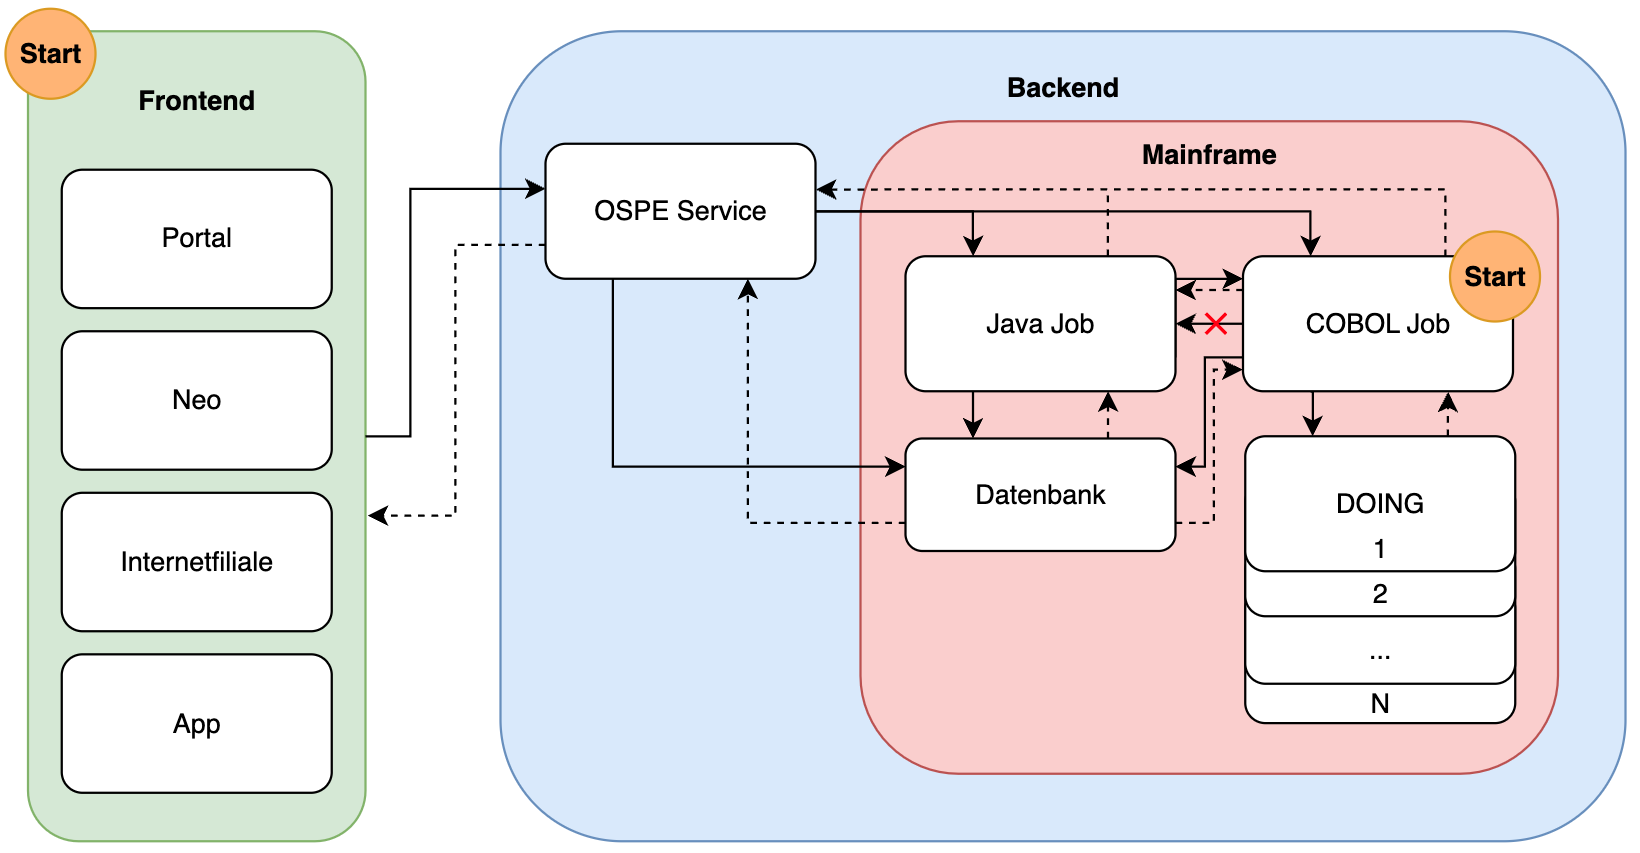
\includegraphics[width=0.9\textwidth]{Abbildungen/OSPlus-Diagramm.png}
    \caption{OSPlus-Diagramm}
\end{figure}

\todo[color=REVIEW]{Itemize notwendig? Ja, bitte}
\begin{itemize}
    \item Ein Mitarbeiter oder ein Endkunde setzt einen Prozess im Frontend in Gang (bspw. Überweisung oder Abfrage eines Kontostands).
    Dies kann über das Portal oder die Neo-Anwendung für Mitarbeiter oder das Online-Banking / die App für Endkunden geschehen.

    Ein Prozess kann ebenfalls durch einen COBOL-Job in Gang gesetzt werden (bpsw. bei Terminüberweisungen).
    \item Die Anfrage wird von einem OSPE-Service verarbeitet.
    Entweder kann dieser die Anfrage direkt (in in Verbindung mit anderen OSPE-Services) bearbeiten oder er ruft einen Java- oder COBOL-Job auf.
    \item Der Java-Job kann ebenfalls COBOL-Jobs aufrufen, andersherum ist dies nicht möglich.
    \item Bei bestimmten Prozessen (bpsw. Transaktionen) müssen eine Anzahl an Prüfungen - die DOINGs - durchgeführt werden. 
    (Z. B., ob die IBAN existiert, ob der Kontoinhaber der richtige ist, ob das Konto gedeckt ist oder auch, ob der Empfänger auf einer Sperrliste steht.) 
    \item Ist diese Prüfung erfolreich, kann der Prozess fortgesetzt werden.
    \item Sowohl die OSPE-Services als auch die Java- und COBOL-Jobs greifen auf die Datenbank zu, um die benötigten Daten zu erhalten bzw. zu speichern. 
\end{itemize}

Kostentechnisch ist es schwer, die Kosten pro Transaktion zu bestimmen, da es sich hierbei um Volumentverträge handelt.
Den Sparkassen werden 1,00 € bis 1,50 € pro tausend Zahlungsein- oder -ausgängen berechnet.\footnote{Vgl. interne Preisliste OSPlus 2024.}

\bigbreak
\bigbreak

\noindent
Um Daten nachvollziebar zu speichern - also so, dass auch nach Änderung oder eigentlicher Löschung noch der vorherige Stand ermittelbar ist -, werden Daten nie wirklich aktualisiert oder gelöscht, sondern es wird ein neuer Datensatz angelegt, der den aktuellen Stand der Daten enthält.
Der alte Stand wird nur „deaktiviert”, also mit einem Ablaufdatum versehen, sodass dieser nicht mehr verwendet wird.\footappendix{Vgl. hierzu und zum Folgenden}{i1:f2}
Erst nach einer in der DSGVO festgelegten Zeit - im Falle von Kontodaten sind dies 10 Jahre - kann dieser Datensatz dann wirklich gelöscht werden.



\todo[color=REVIEW]{Evtl. noch GPS erklären?}
\noindent

\subsection{DLS als Datenbank}

% \subsubsection{Zahlungsverkehr}

\todoin[color=NOTES]{
Zahlungsverkehr: \break
- Je nach Aufbau kann nur der Kontoinhaber selbst eine Transaktion vornehmen \break
- Transaktionen können nicht rückgängig gemacht werden --> Rückbuchung durch erneute Transaktion \break
- Transaktionen können nicht verändert werden --> Keine Manipulation möglich \break
- AuditLog ist automatisch durch Technologie vorhanden \break
- Durch Smart Contracts können bestimmte Finanzprodukte (z.B. Sparverträge, Kredite, ...) oder auch Multisign (per Multisign Contracts) abgebildet werden und so automatisiert werden \break
Großrechnerabschaffung \break
\break
Probleme: \break
- Transaktionen sind öffentlich einsehbar --> Keine Privatsphäre (außer evtl. durch HD-Wallets) \break
- Euro keine Kryptowährung --> Umwandlung in Token notwendig \break
- Weiterentwicklung bei bspw. neuen Anforderungen schwierig --> Durch Proxys möglich \break
}

\todo[color=REVIEW]{
    Formulierungen überarbeiten
    QUELLEN!?
}
Ein Use Case dieser Technologie in Bereich einer Bank wäre der Zahlungsverkehr. 
So wird die Blockchain als Datenbank für die Konten der Kunden verwendet.
Eine Blockchain erfüllt automatisch durch ihren Aufbau einige Anforderungen an den Zahlungsverkehr, die in herkömlichen Systemen beachtet und umgesetzt werden müssen. 
So können Transaktionen - also in diesem Fall Einträge in diese Datenbank - nicht rückgängig, nicht verändert und so nicht manipuliert werden. 
Es gäbe dennoch die Möglichkeit - je nach konkreter Implementierung - bestimmte Sicherheitsmechanismen einzubauen, um bspw. gegen Geldwäsche oder fehlerhaft Buchungen vorzugehen. \todo[color=TODO]{Ausführlicher \& Besipiele / konkrete Idee der Implementierung}
Außerdem ist ein AuditLog automatisch vorhanden, da alle Transaktionen in der Blockchain gespeichert werden.
Aufbauend darauf können Smart Contracts verwendet werden, um bestimmte Finanzprodukte (z.B. Sparverträge, Kredite, ...) oder auch Multisign (per Multisign Contracts) abzubilden und so zu automatisieren. \todo[color=TODO]{Ausführlicher \& Besipiele / konkrete Idee der Implementierung}
%...
\subsubsection{Datenspeicherung}
Um den Kontostand eines Kunden widerzuspiegeln, gibt es folgende Möglichkeiten.

\paragraph{Layer 1 Währung}
Bei der Darstellung des Kontostandes als Layer 1 Währung (z. B. ETH) müsste jeder Kunde ein Wallet erhalten / besitzen, dass den Wert des Kontos in einer Layer 1 Währung enthält.
Das Problem dabei ist, dass diese nicht den Euro darstellt. 
So müsste der Wert immer in eine andere Währung umgerechnet werden, was zu zusätzlichen Kosten führt. Außerdem ist der Wert einer Layer 1 Währung sehr volatil, was zu Problemen führen kann, wenn der Wert des Kontos nicht mit dem Wert der Layer 1 Währung übereinstimmt.
Die Darstellungsart kommt also nicht in Frage.

\paragraph{ERC20 Token}
\input{Theorie/Definitionen/ERC20-Token.tex}

\bigbreak

\noindent
Es gibt bestimmte ERC20 Token, die den Wert anderer Assets (unter anderem auch den Euro) abbilden. Diese werden Stablecoin genannt.\footcite[Vgl. hierzu und weiterführend][4]{q8}
Das Problem daran - sowie auch bei der Layer 1 Währung - ist, dass diese einen tatsächlichen Wert haben, und so die Bank dieses Geld nicht für eigene Geschäfte verwenden kann.

\bigbreak

\phantomsection
\label{datenspeicherung:neuer-token}
\noindent
Es wäre also die Erstellung eines eigenen Tokens sinnvoll, um den Wert eines Kontos darzustellen, ohne dass dieser einen tatsächlichen Wert hat. So kann die Bank diesen Wert für eigene Geschäfte verwenden, ohne dass der Kunde dadurch einen Verlust erleidet. 
Außerdem kann so gewährleistet werden, dass nur Kunden der Bank diesen Token verwenden können, da die Bank die einzige ist, die diesen Token ausgibt.
Außerdem muss der erstellte Token nicht zwingend die genauen Schnittstellen eines ERC20 Tokens, sondern lediglich die Anforderungen der Bank erfüllen.

\todo[color=TODO]{
    Schwierigkeit der Datenlöschung (im Sinne DSGVO)
    - Möglickeit durch Löschung des Indexes

    ... Index und sensible Daten können entweder verschlüsselt oder zentral gespeichert werden
}

\input{Zahlungsverkehr/Datenbank/Anonymität.tex}

\todo[color=REVIEW]{Wohin mit dem Abschnitt?}
\noindent

\subsubsection{Öffentliche vs. private Chain}
\label{sec:oeffentlich-vs-privates-netzwerk}

\todoin[color=NOTES]{
    Öffentliches vs. privates Netzwerk: \break
    PRivates: \break
    - Nur für bestimmte Teilnehmer (in dem Falle dann nur FI) \break
    - wirds wirklich nur von einer Authority verwendet können die Daten geändert werden \break
    - "eigene" Regeln (bspw. kein Gas) \break
    \break
    Öffentliches: \break
    - Anonymität schwierig zu gewährleisten \break
    - Transaktionskosten \break
    - Daten können nicht geändert werden \break
}

Bei der Verwendung einer Blockchain gibt es die Möglichkeit, einer öffentlichen Chain „beizutreten“ oder dafür eine private Chain zu betreiben.\footcite[Vgl.][]{w10}
Eine öffentliche Chain ist für alle Teilnehmer offen und kann von jedem verwendet werden.\footcite[Vgl. hierzu und zum Folgenden][]{w11}
Eine privatee Chain hingegen ist nur für ausgewählte Teilnehmer zugänglich und wird i.d.R. von einer oder mehreren Organisationen / Unternehmen betrieben.
Die Auswahl der Art der Chain kann an den Punkten Sicherheit / Unveränderlichkeit, Leistung, Kosten, Berechtigungen und Datenschutz / Anonymität erfolgen:
\begin{itemize}
    \item \textbf{Sicherheit / Unveränderlichkeit:} 
    \todo[color=REVIEW]{Folgendes eher in Definition oder späterer Analyse?}
    Die Sicherheit und Unveränderlichkeit einer Blockchain wird durch ihren Konsensalgorithmus bestimmt. 
    Eine öffentliche Chain wird durch die Interaktion von Tausenden unabhängigen Nodes gesichert, die von Einzelpersonen und Organisationen auf der ganzen Welt betrieben werden. 
    Private Chains haben typischerweise eine kleine Anzahl von Nodes, die von einer oder wenigen Organisationen kontrolliert werden. 
    Diese Nodes können streng kontrolliert werden, aber nur wenige müssen kompromittiert werden, um die Chain umzuschreiben oder betrügerische Transaktionen durchzuführen.

    \item \textbf{Leistung:} 
    Bei privaten Chains können Hochleistungsnodes mit besondererer Hardware sowie ein anderer Konsensalgorithmus verwendet werden, um einen höheren Tansaktionsdurchsatz auf der Basisschicht (Layer 1) erreichen.
    Bei einer öffentlichen Chain kann ein hoher Durchsatz mit Hilfe von Layer 2 Skalierungslösungen erreicht werden.

    \item  \textbf{Kosten:}
    Die Kosten für den Betrieb einer privaten Chain spiegeln sich hauptsächlich in der Arbeit wider, die Chain einzurichten und zu verwalten, und den Servern zu betreiben, auf denen sie läuft. 
    Während es keine Kosten gibt, um sich mit dem Ethereum Mainnet zu verbinden, muss die Gas Fee (s. \ref{sec:definition-gas-fee}) für jede Transaktion in Ether bezahlt werden.
    Abhilfe können Transaction Relayers (s. \ref{sec:definition-transaction-relayers}) sein, sodass ein Endkunde diese Gebühr nicht selbst tragen muss.

    Einige Analysen haben gezeigt, dass die Gesamtkosten für den Betrieb einer Anwendung auf einer öffentlichen Chain niedriger sein können als beim Betrieb einer privaten Chain.\footcite[Vgl.][14]{q6}
    \todo[color=REVIEW]{Die Quelle genauer erläutern?}

    \item \textbf{Berechtigungen:}
    Bei privaten Chains können nur autorisierte Teilnehmer Nodes einrichten und Transaktionen durchführen.
    Bei öffentlichen Chains kann jeder Node einrichten und Transaktionen durchführen.
    So kann ebenfalls jeder auf jeden Contract zugreifen, also dessen gespeicherte Daten auslesen und Funktionen aufrufen.
    Daher müssen erstellte Contracts so implementiert werden, dass sie nur von den gewünschten Teilnehmern verwendet werden können (s. \ref{sec:definition-sicherheitsrisiken}).

    \item \textbf{Datenschutz / Anonymität:}
    Der Zugang zu Daten, die auf privaten Chains festgehalten wurden, kann frei vom Betreiber kontrolliert werden. 
    Alle Daten, die auf einer öffentlichen Chain geschrieben wurden, sind für jeden einsehbar, so dass sensible Informationen off-chain gespeichert und übertragen  oder verschlüsselt werden sollten. 
    Es bestehen Designpattern, die dies erleichtern, sowie Layer 2 Lösungen, die Daten abgetrennt und von Layer 1 fernhalten können (s. \ref{sec:definition-layer-2-solutions}).

    Ebenso sind alle Transaktionen auf einer öffentlichen Chain öffentlich einsehbar, sodass die Anonymität der Teilnehmer nicht gewährleistet werden kann (s. \ref{sec:definition-account-based-vs-utxo-based-chain}).
\end{itemize}

% \input{Theorie/Definitionen/Transaction-Relayers.tex}

\input{Theorie/Definitionen/Sicherheitsrisiken.tex}

\todoin[color=TODO]{
Fazit / Empfehlung welche Chain verwendet werden soll \break
--> Öffentlich, da sonst nicht dezentral und so unsicher (Änderung der Daten möglich / also quasi gleiches System wie jetzt)\break

Grundsätzlich viele Vorteile bei privater Chain (evtl. dann im Kontext, wenn mehrere Banken dies benutzen)

}

\subsubsection{Transaktionskosten und -durchsatz}
Ethereum kann nur eine geringe Anzahl an Transaktionen pro Sekunde (ca. 20TPS bis 30TPS)  verarbeiten\footcite[Vgl.][]{w36}, daher liegen die Transaktionskosten je nach Netzwerkauslastung zwischen ca. \$2 bis \$20\footcite[Vgl.][]{w35}.
Um die Skalierbarkeit zu erhöhen und Transaktionskosten zu senken, werden Layer 2 Lösungen eingesetzt.\footcite[Vgl.][]{w17}

\input{Theorie/Definitionen/Layer2-Solution.tex}

\bigbreak
\noindent
Um mit dem hohen Datenvolumen der Sparkassen fertigzuwerden, müssen Layer 2 Lösungen verwendet werden. 
Wobei auch hier fraglich ist, ob diese der Masse an Transaktionen standhalten können (es wird mit ca. 100.000 TPS gerechnet).\footcite[Vgl.][]{w34}
Preislich soll eine Transaktion weitaus weniger als \$0,1 kosten.\footcite[Vgl.][]{w37}


\input{Theorie/Definitionen/Transaction-Relayers.tex}

\bigbreak
\noindent
Transaction Relayers wären sinnvoll, wenn ein Kunde selbst über das Netzwerk bpsw. Überweisungen o. ä. durchführen kann.
Da allerdings nur die FI selbst Transaktionen durchführt - ein Endkunde würde dann durch die Services der Sparkassen und so der FI das System verwenden - und diese selbst die Kosten für die Transaktionen tragen muss, ist es nicht notwendig Transaction Relayers zu verwenden.
\subsection{DLS als Mainframersatz}
Um den Mainframe wirklich ablösen zu können, reicht es nicht aus lediglich die Datenbank zu ersetzen.
Es muss auch die Verarbeitung und Prüfung der Daten übernommen werden.
Kurzum müssen also die COBOL- und Java-Jobs sowie die DOINGs, die akutell auf dem Mainframe laufen, ersetzt werden.

\noindent
Eine Möglichkeit wäre es, all diese Jobs durch Smart Contracts zu ersetzen.
Allerdings wären so alle Verarbeitungen und Prüfungen öffentlich einsehbar, was sensible Daten (wie bspw. Name oder IBAN) offenlegen würde.
Außerdem wäre dies durch die Transaktionskosten sehr teuer.

\noindent
Da durch das hohe Datenaufkommen der Sparkassen die Verarbeitung der Daten sehr performant sein muss, ist es ebenfalls nicht möglich, die Verarbeitung der Daten auf der Blockchain selbst durchzuführen.
Wie bereits beschrieben muss also eine Layer 2 Lösung verwendet werden (s. \ref{sec:definition-layer-2-solutions}).
Da die FI die einzige Instanz ist, die Transaktionen durchführt und so keine gesonderte Prüfung der Transaktionen notwendig ist, bietet sich hier ein (modifiziertes) Optimistic Rollup an. 
(Die Challange-Periode ist nicht erforderlich, es wird also immer der durch das Rollups kreierte Batch verwendet.)
Die FI wickelt also den Zahlungsverkehr weiterhin auf eigenen Systemen ab und übersendet nur die Ergebnisse an die Layer 1 Chain.
So werden die Prüfungen und Verarbeitungen der Daten auch nicht öffentlich ausgeführt und sind nicht einsehbar.

\noindent
Bestimmte Finanzprodukte lassen sich dennoch gut durch Smart Contracts abbilden und so automatisieren.
Darunter zählen z. B. automatische Zinsvergaben am Monats- oder Jahresabschluss oder auch Termin- oder Daueraufträge.

\subsubsection{Optimistic Rollups in Verbindung mit Cloud Computing}
Eine mögliche Alternative den Mainframe abzulösen, ist die Verwendung von Cloud Computing.
Cloud Computing wird nach dem National Institute of Standards and Technology durch die folgenden fünf Eigenschaften definiert:\footcite[Vgl. hierzu und zum Folgenden][5]{q11}
\begin{itemize}
    \item \textbf{On-Demand Self-Service:} 
    Der Nutzer kann die benötigten Ressourcen (bspw. Rechenleistung, Speicherplatz, etc.) selbstständig und ohne menschliche Interaktion mit dem Anbieter bereitstellen.
    \item \textbf{Broad Network Access:}
    Die Ressourcen sind über das Netzwerk verfügbar und können von verschiedenen Plattformen (bspw. Desktop, Laptop, Smartphone, etc.) abgerufen werden.
    \item \textbf{Resource Pooling:}
    Die Ressourcen des Anbieters werden gebündelt und können so von mehreren Nutzern verwendet werden.
    \item \textbf{Rapid Elasticity:}
    Die Ressourcen können schnell und dynamisch an die Bedürfnisse des Nutzers angepasst werden.
    \item \textbf{Measured Service:}
    Die Nutzung der Ressourcen wird quantitativ und qualitativ überwacht, so dass eine nutzungsabhängige Abrechnung sowie eine Validierung der Dienstqualität möglich ist.
\end{itemize}

\noindent
Der größte Vorteil für die FI wäre hier die gute Skalierbarkeit der Ressourcen und die nutzungsabhängige Abrechnung.
\bigbreak
\noindent
Ein größer Nachteil dieser Technologie ist die Datensicherheit, da sich diese in der Hand des Anbieters befindet und so nicht kontrolliert werden kann.\footcite[Vgl. hierzu und zum Folgenden][99]{q10}
Es besteht generell keine Kontrolle über die Art und Weise der Speicherung.
So ist ein Wechsel des Anbieters sehr aufwendig, da die Daten möglicherweise nicht einfach migriert werden können.\footcite[Vgl.][]{w28}

\noindent
Hier können DLS Abhilfe schaffen.
So können die Optimistic Rollups auf einem Cloud System ausgeführt, die Daten aber dennoch in der Blockchain gespeichert werden.
So sind sie tranzparent und nach eigenen Vorstellungen gespeichert, aber die Verarbeitung der Daten kann auf einem Cloud System erfolgen.
Darüber hinaus können die Daten nicht nur vom verwendeten Anbieter selbst aus eingesehen werden - da sie sich im öffentlcihen Netzwerk befinden - und eine Migration ist so einfacher möglich.
Man ist also nicht stark an einen Anbieter gebunden.

\subsubsection{Erweiterbarkeit}
\label{sec:Erweiterbarkeit}

Sollten Finanzprodukte in Smart Contracts umgesetzt werden oder sich die Funktionsweise der Optimistic Rollups in Zukunft ändern, ist es wichtig, dass diese Funktionen erweiterbar / weiterentwickelbar sind.
Die Grundidee einer Blockchain basiert allerdings darauf, dass einmal geschriebene Daten - und so auch Smart Contract - nicht mehr verändert werden können (sie sind „immutable”).\footcite[Vgl.][]{w30}
Es gibt drei Möglichkeiten, wie Smart Contracts erweitert werden können:\footcite[Vgl. hierzu und zum Folgenden sowie weiterführend][]{w29}
\begin{itemize}
    \item \textbf{Contract Migration:}
    Bei der Contract Migration löst ein neuer Contract den alten ab.
    Alle Daten, die im alten Contract gespeichert wurden, müssen also in den neuen Contract übertragen werden.
    Die Datamigration ist meist sehr aufwendig und mit hohen Gas-Kosten verbunden.

    \item \textbf{Data Seperation:}
    Bei der Data Seperation werden Daten und Logik in zwei verschiedene Contracts aufgeteilt.
    So kann der „Logik-Contract” ersetzt werden, ohne dass die Daten migriert werden müssen.
    Hier müssen aufwendige Sicherheitsmaßnahmen getroffen werden, um zu gewährleisten, dass nur der Logik-Contract die Daten verändern kann.

    \item \textbf{Proxy:}
    Bei der Verwendung eines Proxys wird ein zusätzlicher Contract verwendet, der als Schnittstelle zu dem eigentlichen Contract dient.
    Es ist möglich, dass ein Contract die Funktionen eines anderen Contracts in seinem Kontext - also mit seinem Speicher - aufruft.
    Der Proxy Contract hält also den Speicher, während der dahintergeschaltete Contract die Logik enthält.
    So kann der Proxy Contract einfach ausgetauscht werden, ohne dass die Daten migriert werden müssen.

    \noindent
    Bei Proxys gibt es mehrere Architekturen, die sich in der Art und Weise, wie der Proxy mit dem dahintergeschalteten Contract interagiert, unterscheiden.
    Häufig kommt zusätzlich ein Admin Contract zum Einsatz, der die Berechtigung hat, den Logik-Contract zu ändern.
\end{itemize}

\noindent
Da mehrere Finanzprodukte in Smart Contract abgebildet werden könnten, bietet es sich an für jedes Produkt einen eigenen Contract zu verwenden und diese dann über einen gemeinsamen Proxy anzusprechen.

    \noindent

\section{Schlussfolgerung}
\label{sec:Fazit}

Die Verwendung von DLS also reine Datenbank verfehlt den Zweck, den Großrechner abzulösen. 
Hinzu kommt, dass die Verwendung als Datenbank auch keine sonderlich gute Alternative ist, da dies mit einem sehr hohem Aufwand und Komplexität verbunden ist und die Verwendung teurer und langsamer ist.
Außerdem besteht auch kein Problem mit der aktuellen Art und Weise wie Daten gespeichert werden, dass mit DLS gelöst werden würde.

\noindent
Die Verwendung von Optimistic Rollups als Ersatz für den Großrechner ist schon eher eine Alternative, allerdings auch sehr komplex.
Die Verwendung von DLS in Verbindung mit Cloud Computing könnte allerdings eines der größten Probleme, die mit Cloud Computing bestehen - die Datensicherheit -, lösen.
Allerdings ist es fraglich, ob diese Technologie die Performance des Großrechners erreichen kann.
Dafür müsste diese Idee prototypisch umgesetzt und getestet werden, was aufgrund der hohen Komplexität und des benötigten Testdatenumfangs mit einem sehr hohen Aufwand verbunden wäre.
%Es bestehen hohe Zweifel, ob andere Technologien den Großrechner ersetzen können.\footappendix{Vgl.}{i1:f4}

\noindent
Daher ist die Verwendung von DLS für den Zahlungsverkehr der Sparkassen eher wenig geeignet.
Wenn, dann nur in Verwendung mit Cloud Systemen.
\noindent

\section{Ausblick}
\label{sec:ausblick}

Die grundlegende Idee eines DLS ist es, dessen Teilnehmer zu vernetzen, ohne zentrale Instanzen zu verwenden und so kein Vertrauen in diese setzen zu müssen (s. \ref{sec:definition-kryptowaehrung}).
Da in dieser Arbeit die Verwendung von DLS lediglich im Scope einer einzelnen Instanz - der FI - betrachtet wurde, und daher keine Vernetzung stattfindet, fällt dieser Vorteil vollständig weg.
Eine weitaus sinnvollere Verwendung im Berech Zahlungsverkehr wäre die Vernetzung mehrerer Banken, um so bpsw. Transaktionen auszuführen.
Dafür kann auch ein privates Netzwerk geschaffen werden, da dies dann auch dezentral wäre und so die Vorteile eines DLS genutzt werden können.
Die Bundesbank hat hierzu einen Bericht geschrieben, in dem sie sich positiv für diese Technologie im Auslandszahlungsvekehr äußert, um diesen so zu vereinfachen und zu beschleunigen. \footcite[Vgl.][44]{q12}
    \newpage

    % \input{Grundlagen Netzwerk.tex}

    % \input{Grundlagen UI.tex}

    % \input{Grundlagen Frameworks.tex}

    % \input{Methodik.tex}

    % \input{Anwendung.tex}

    % \input{Mängel.tex}

    % \input{DV.tex}

    % \input{neuFR.tex}

    % \noindent

\section{Ausblick}
\label{sec:ausblick}

\todoin[color=NOTES]{
Implemetierungsideen: \break
- HD-Wallets / UTXO-Token \break
- Proxys \break
- Transaction Relayers \break
\break
Weitere Ideen: \break
- Einbindungen mehrerer Banken --> Privates Netzwerk schaffen (So wie bei Bundesbank beschrieben) \break
- Durch Optimitic Rollups Mainframe ersetzen \break
\break
\break
Formulierungen:\break
... genaueres kann nur eine wirklich praktische Umsetzung / Implementierung zeigen\break

Es bestehen hohe Zweifel, dass andere Technologien den Großrechner ersetzen können. --> Christian \break
}

    % \section{Schlussfolgerung}
\label{sec:Fazit}

Die Verwendung von DLS also reine Datenbank verfehlt den Zweck, den Großrechner abzulösen. 
Hinzu kommt, dass die Verwendung als Datenbank auch keine sonderlich gute Alternative ist, da dies mit einem sehr hohem Aufwand und Komplexität verbunden ist und die Verwendung teurer und langsamer ist.
Außerdem besteht auch kein Problem mit der aktuellen Art und Weise wie Daten gespeichert werden, dass mit DLS gelöst werden würde.

\noindent
Die Verwendung von Optimistic Rollups als Ersatz für den Großrechner ist schon eher eine Alternative, allerdings auch sehr komplex.
Die Verwendung von DLS in Verbindung mit Cloud Computing könnte allerdings eines der größten Probleme, die mit Cloud Computing bestehen - die Datensicherheit -, lösen.
Allerdings ist es fraglich, ob diese Technologie die Performance des Großrechners erreichen kann.
Dafür müsste diese Idee prototypisch umgesetzt und getestet werden, was aufgrund der hohen Komplexität und des benötigten Testdatenumfangs mit einem sehr hohen Aufwand verbunden wäre.
%Es bestehen hohe Zweifel, ob andere Technologien den Großrechner ersetzen können.\footappendix{Vgl.}{i1:f4}

\noindent
Daher ist die Verwendung von DLS für den Zahlungsverkehr der Sparkassen eher wenig geeignet.
Wenn, dann nur in Verwendung mit Cloud Systemen.

    % \newpage

    %==================================================
    %Quellen
    %==================================================

    \defbibheading{bibnumbered}[Quellenverzeichnis]{
        \section{#1}
    }
    \printbibliography[heading=bibnumbered]

    \newpage


    %==================================================
    %Anhangsverzeichnis 
    %==================================================

    %Seitennummerierung mit römischen Zahlen
    \pagenumbering{Roman}
    %letzte römische Seite wird gespeichert und hier weitergeführt
    \setcounter{page}{\numexpr\value{romanPage}+1}

    \appendix
    % Kapitelnummerierung fortsetzen IV, ...
    \setcounter{section}{\theromanSection}
    \renewcommand{\thesection}{\Roman{section}}

    \parindent0mm

    \section{Anhangsverzeichnis}

    \newcommand{\listappendicesname}{Anhangsverzeichnis}
    \renewcommand{\listappendicesname}{}
    \newlistof{appendices}{apc}{\listappendicesname}


    \newcommand{\appendices}[1]{\addcontentsline{apc}{appendices}{#1}}

    % \GetTitleStringSetup{expand}
    \newcounter{appendix}

    \titleformat{\subparagraph}
    {\normalfont\normalsize\bfseries}{Anhang \arabic{appendix}{ - }}{0em}{}

    \newcommand{\newappendix}[1]{
      \phantomsection
      \stepcounter{appendix}
      % \refstepcounter{appendix}
      \appendices{Anhang \arabic{appendix} - #1}
      \subparagraph{#1}
    }

    \listofappendices

    \newpage


    %==================================================
    %Anhang
    %==================================================
    \section{Anhang}
    \titleformat*{\section}{\fontsize{12}{14}\selectfont\bfseries} % Schriftgröße und Zeilenabstand ändern
    \setcounter{page}{1}
    \renewcommand{\thepage}{A\arabic{page}}

% ==================================================
% Anhang
% --------------------------------------------------

\newappendix{Interviewleitfaden für das Interview mit Christian Krauthoff}
\label{Interviewleitfaden für das Interview mit Christian Krauthoff}

\todo[color=TODO]{Intervierwleitfaden schreiben}
\begin{tabular}{|p{10cm}|p{4cm}|}
    \hline
    \textbf{Interviewfragen} & \textbf{Bezugskapitel} \\
    \hline
    1. Frage 1 & Kapitel 1 \\
    \hline
    2. Frage 2 & eigene Ergänzung \\
    \hline
    \end{tabular}

\newpage

\newappendix{Interviewprotokoll 1: Christian Krauthoff}\label{appendix: Anhang 3}

\todo[color=REVIEW]{Daten überprüfen}
\begin{tabular}{p{2.5 cm}p{11.8 cm}}
\textbf{Protokoll:} & Gespräch mit Christian Krauthoff \\
\textbf{Teilnehmer:} & Christian Krauthoff - Abteilungsleiter AZV \& ZV-Rekla (OE-4293) \break Tobias Binnewies - Dualer Student \\
\textbf{Thema:} & Produktionsdatenspeicherung / Transaktionskosten / Großrechner \\
\textbf{Dauer:} & 30 min
\end{tabular}
\bigbreak
\noindent\rule[1ex]{\textwidth}{1pt} %Linie
\bigbreak

\textbf{Frage:} 
\phantomsection
\label{i1:f1}
Wie wird sichergestellt, dass Produktionsdaten (bspw. Kontodaten) nicht manipuliert werden können?


\textbf{Antwort:} 
Als Mitarbeiter braucht man ein Produktionsrecht und ein recht sensitive Daten einsehen zu dürfen, um auf die Daten mit einem Auftragsgrund zugreifen zu können. Der Auftragsgrund besteht dann durch ein Ticket, also quasi eine „Beschwerde” durch ein Institut.
Nur dann kann ein FI-Mitarbeiter auf Produktionsdaten zugreifen.
Um Daten abzuändern muss noch ein weiteres Recht beantragt werden, das nur wenige Mitarbeiter haben.
Außerdem kommt das Vieraugenprinzip zum Einsatz, sodass immer mindestens zwei Mitarbeiter mit diesem Recht das SQL-Statement einsehen müssen, bevor es ausgeführt wird.

Source Code wird maschinell geprüft, also bspw. dass keine festen IBANs, Namen oder ähnliches im Code fest abgefragt werden.
Außerdem wird immer ein Code Review von „Unabhängigen„ - also Entwicklern, die an diesem Projekt nicht beteiligt waren - durchgeführt, um so die Qualität des Codes zu gewährleisten.

\bigbreak
\bigbreak

\textbf{Frage:}
\phantomsection
\label{i1:f2}
Wie werden Daten bei Änderung nachvollziehbar gespeichert?


\textbf{Antwort:}
Wenn Daten „gelöscht” werden oder auch geändert werden, werden diese nie wirklich gelöscht sondern nur deaktiviert.
So gibt es bei jeder gespeicherten Zeile in der Datenbank ein Feld „Gültig bis”, welches erst einmal leer ist. 
Ändert sich nun etwas an der Zeile, wird das Feld „Gültig bis” mit dem Datum der Änderung gefüllt und eine neue Zeile mit den neuen Daten wird angelegt.
So ist eine Löschung oder Änderung jederzeit nachvollziehbar.

In der DSGVO ist festgelegt, sind Datenlöschungfristen festgelegt.
Kontodaten haben eine Löschfrist von 10 Jahren, d. h. diese müssen 10 Jahre lang gespeichert werden und können dann erst wirklich gelöscht werden.

\bigbreak
\bigbreak

\textbf{Frage:}
\phantomsection
\label{i1:f3}
Wie hoch sind die Kosten pro Transaktion?


\textbf{Antwort:} 
Die Informationen dazu stehen im Produktkatalog. Außerdem gibt es SQLs, die einem die genauen Kosten für das jeweilige Insitut auswerfen.

Die Kosten für die Finanz Informatik sind pro Transaktion schwer anzugeben, da es sich hierbei um Volumentverträge handelt. 
Hierbei wird eine Lastspitze der Großrechners im gesamten Jahr festgelegt und demnach abgerechnet. 


\bigbreak
\bigbreak

\textbf{Frage:}
\phantomsection
\label{i1:f4}
Gibt es Projekte um vom Großrechner wegzukommen?


\textbf{Antwort:}
Ja, man möchte klar vom Großrechner wegkommen - und auch vorallem von IBM abhängig zu sein.
Es gibt das Projekt „COBOL to Java”, also von COBOL / IBM weg und so nur noch die kritischen Themen dort zu halten, also im Rahmen von Zeit und Massendatenverarbeitung und den Rest alles auslagern in Java.
Allerdings laufen die Java-Jobs zum Teil auch auf dem Großrechner, das Zeil ist jedoch - sofern möglich - die Großrechnerjobs immer weiter zu reduzieren.

Das Problem ist immer die Geschwindigkeit und Massendaten, da dies durch kein anderes System so gut abbildbar ist wie durch den Großrechner.
Bspw. schafft der Großrechner, wenn ein Job mit ca. 1,4 Millionen Transaktionen anstartet ca. 20 Sekunden.
Oder auch wenn z. B. die DKB am Monatsende mit ihren ca. 1,8 Millionen Konten Zinsrechnung, Abschußschreibung oder auch Umbuchung durchführt, laufen mehrere Jobs parallel.
Das ist mit anderen Systemen schwer abbildbar, bzw. auch schnwer einmal zu testen.

\bigbreak
\bigbreak

\textbf{Frage:}
\phantomsection
\label{i1:f5}
Was sind Geschäftsprozesse?


\textbf{Antwort:}
Geschäftsprozesse sind quasi ein „Fahrplan”, dort steht drin, was bspw. von der Erfassung bis zur Buchung mit den Daten passiert, also ob z. B. ob aus 5€ noch 15€ werden, da es noch Gebühren gibt oder ist das nicht erlaubt.
Es wird genau geregelt, welcher Prozess wann, wie und in welcher Reihenfolge abläuft.
So kann genau nachgewiesen werden, was genau mit den Daten passiert ist.
Es gibt dann „Datenflussdiagramme„ für einen genauen Prozess um bspw. bei Beschwerde genau nachvollziehen zu könnne, warum was genau passiert ist.
Es ist technisch nicht möglich einen Prozess zu umgehen, da die Daten immer durch die Prozesse laufen.
Außerdem können bpsw. keine Daten gelöscht oder abgeändert werden, wenn dies nicht im Geschäftsprozess vorgesehen ist.

\newpage

\newappendix{OSPlus-Diagramm}
\phantomsection
\label{a1}
\todo[color=TODO]{Quelle einfügen}
\begin{figure}[ht]
    \centering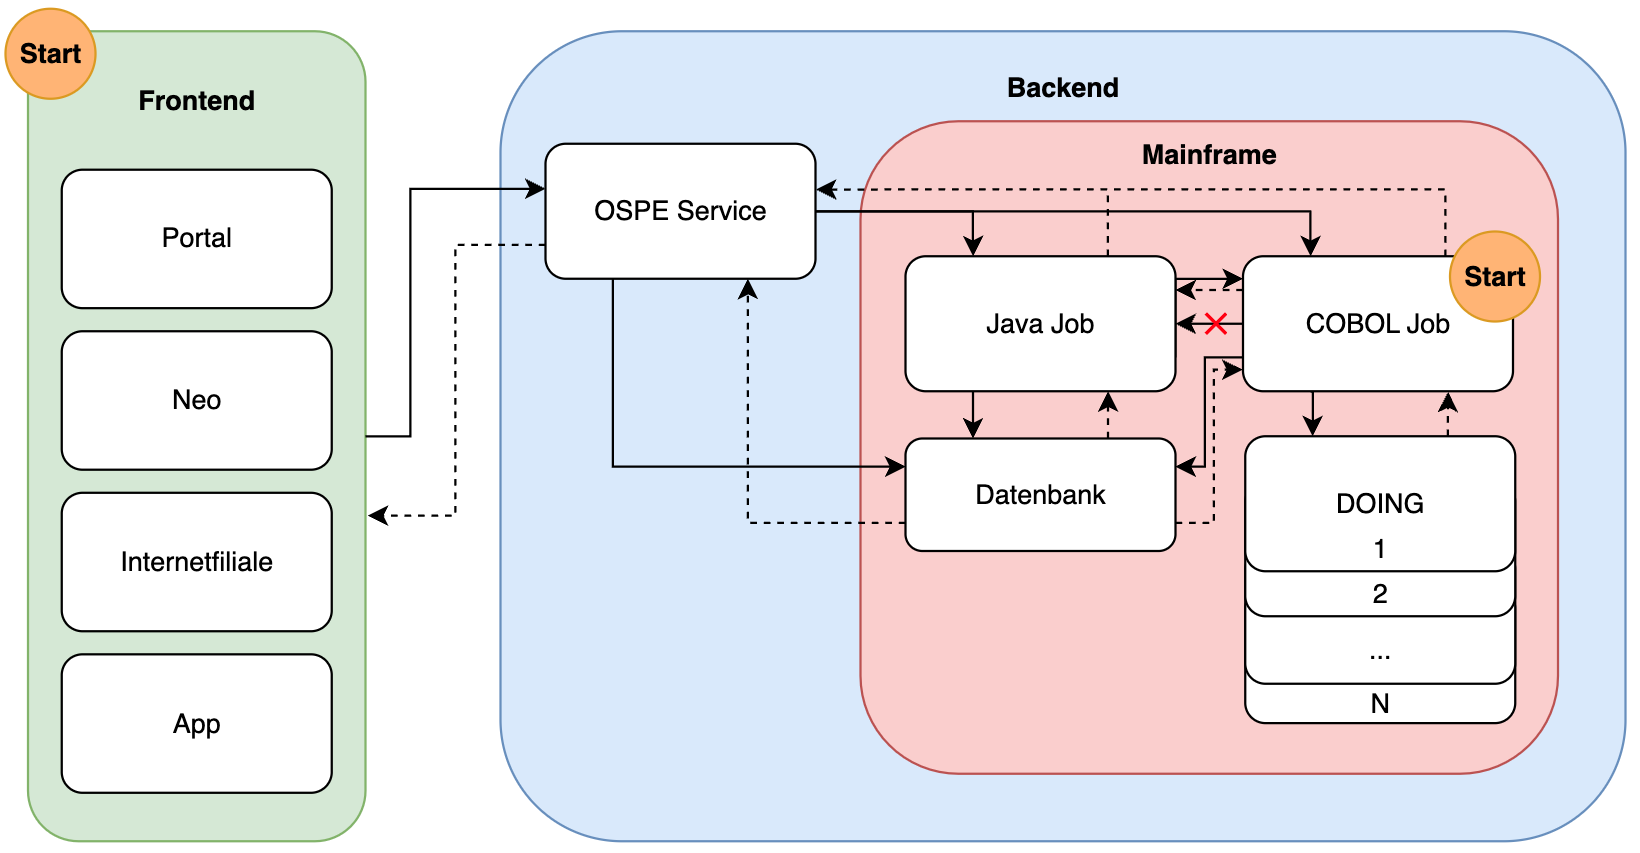
\includegraphics[width=1.0\textwidth]{Abbildungen/OSPlus-Diagramm.png}
\end{figure}

\newpage

\bigbreak
    

\end{document}